\documentclass[review,authoryear]{elsarticle}
\usepackage[T1]{fontenc}
\usepackage{haldefs}
\usepackage{textcomp}
\usepackage{color}
\usepackage[vlined,ruled]{algorithm2e}
\usepackage{array}
\usepackage{multirow}
\usepackage{booktabs}
\usepackage[table]{xcolor}
\definecolor{lightgray}{gray}{0.9}

\begin{document}

\begin{frontmatter}
  \title{A Functional Networks Estimation Method of Resting-State fMRI Using a
    Hierarchical Markov Random Field}

  \author[sci]{Wei Liu}
  \ead{weiliu@sci.utah.edu}

  \author[sci]{Suyash P. Awate}
  \ead{suyash@sci.utah.edu}

  \author[rad]{Jeffrey S. Anderson}
  \ead{andersonjeffs@gmail.com}

  \author[sci]{P. Thomas Fletcher}
  \ead{fletcher@sci.utah.edu}

  \address[sci]{Scientific Computing and Imaging Institute, University of
  Utah, USA}

  \address[rad]{Department of Radiology, University of Utah, USA}

  \begin{abstract}
  We propose a hierarchical Markov random field model for estimating both group
  and subject functional networks simultaneously. The model takes into account
  the within-subject spatial coherence as well as the between-subject
  consistency of the network label maps. The statistical dependency between
  group and subject networks acts as a regularization, which helps the network
  estimation on both layers. We use Gibbs sampling to approximate the posterior
  density of the network labels and Monte Carlo expectation maximization to
  estimate the model parameters. We compare our method with two alternative
  segmentation methods based on K-Means and normalized cuts, using synthetic and
  real fMRI data. The experimental results show our proposed model is able to
  identify both group and subject functional networks with higher accuracy on
  synthetic data, more robustness, and inter-session consistency on the real
  data.
  \end{abstract}

  \begin{keyword}
    resting-state functional MRI, segmentation, functional connectivity,
    hierarchical Markov random field, Bayesian
  \end{keyword}
\end{frontmatter}

\section{Introduction}
To study the intrinsic activity of human brain with resting-state functional MRI
(rs-fMRI) data, one models either the data of a single subject or a group of
subjects. The fMRI image of a single subject is often contaminated with the
noise of various sources, and the results from it are typically unreliable.  On
the other hand, combining data from multiple subjects and estimating the
common functional networks is more robust. Group analysis of rs-fMRI assumes
that all subjects in the group share certain amount of functional connectivity
patterns, and assumes that these group networks can be estimated more accurately
by aggregating the data from all subjects. In practice, it is a major challenge
to summarize the shared patterns across subjects, as the network structure of
each subject appears similar but has fair amount of variations.

\begin{figure*}[htb]
  \centering
  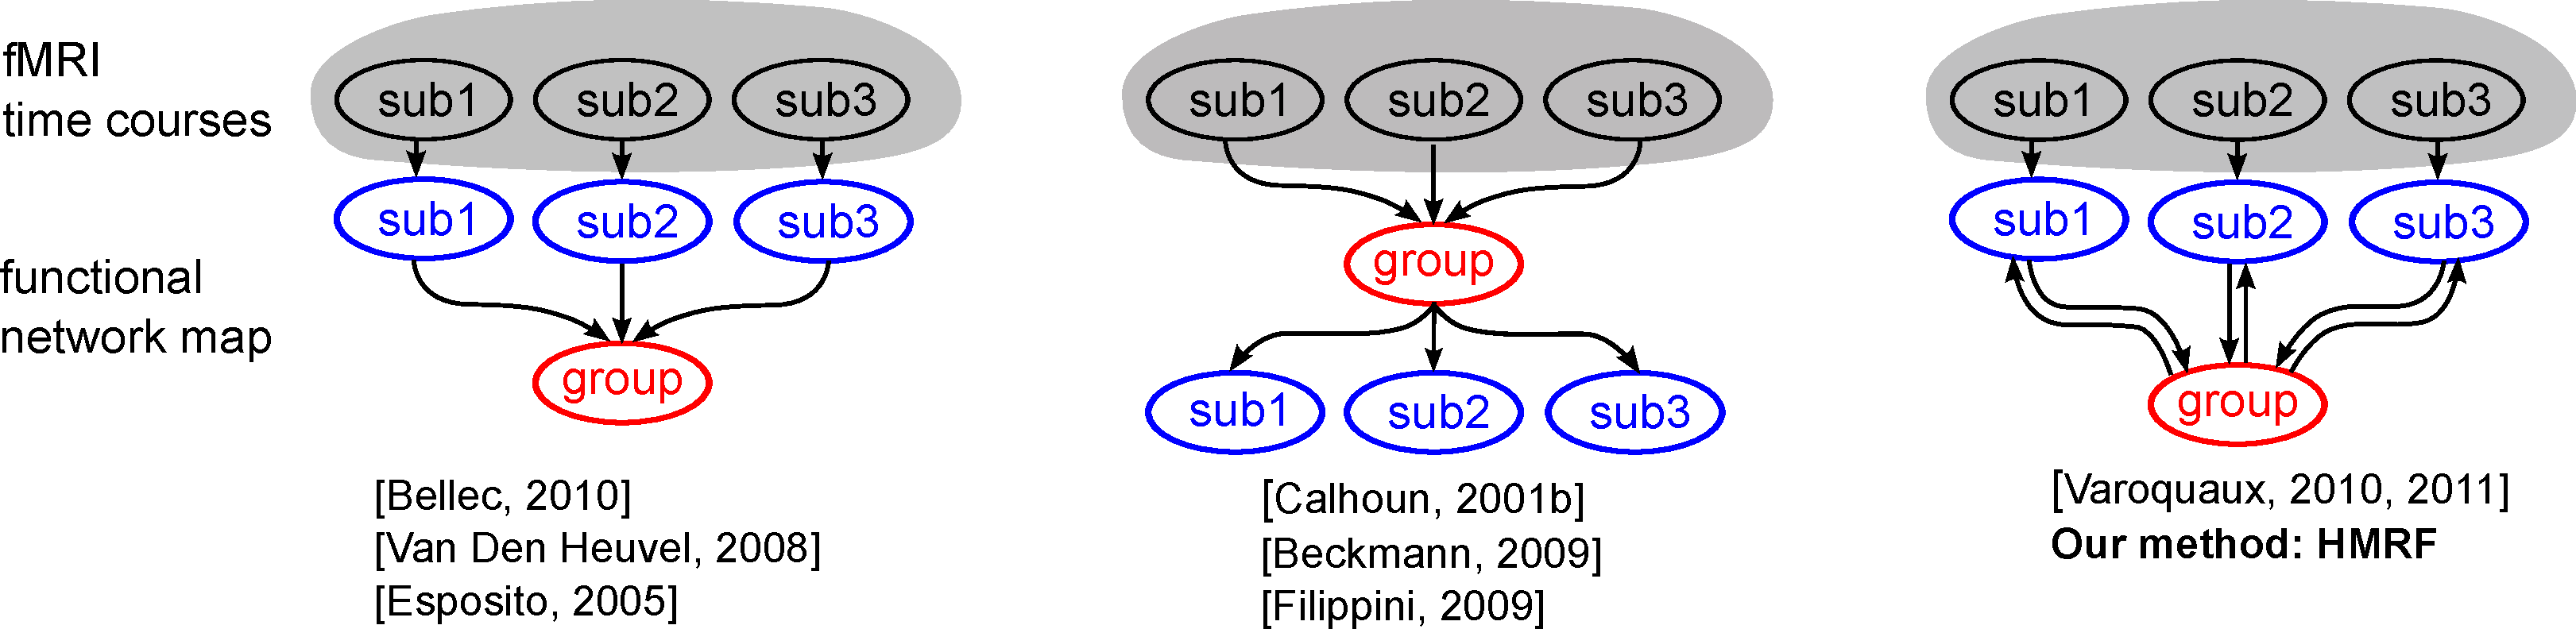
\includegraphics[width=0.9\textwidth]{figures/bidirections/bidirections}
  \caption{Comparison of segmentation methods for group study of rs-fMRI. Most
    methods use a one-way approach, either in a subject-group order (left) or a
    group-subject order (middle). Our method (right) aims at a joint estimation
    of both levels of network maps, where group and subject maps help each other
    in a bidirectional flow}
  \label{fig:bidirections}
\end{figure*}

Recent years have seen substantial interest in estimating functional networks of
individual subjects with the network map of other subjects as a
constraint~\citep{beckmann2009group, varoquaux2011multi, ng2012modeling,
  ng2012group}. An accurate estimate of an individual's network is an important
step towards the understanding of brain-behavior relationships on a per-subject
basis, the identification of the possible correlation between the network
patterns and clinical variables, and the subject-specific treatment. The
explicit modeling of intersubject variation is a key step for a reliable
estimate of single subject as well as the group networks.  Current
methods~\citep{yeo2011organization, damoiseaux2006consistent} either do not
estimate individual functional network maps, or do not have an explicit
statistical model on the intersubject variations~\citep{calhoun2001method,
  calhoun2001spatial}.  Among the methods that do estimate subject functional
networks, some have one or more drawbacks.

First, some methods map a common group functional network by concatenating the
blood oxygen level dependent (BOLD) signal from all subjects. Even the
anatomical structure is perfectly aligned in the co-registration step, the
functional correspondence between subjects is not guaranteed due to the
subject-specific functional localization. In particular, some participants may
experience spontaneous but active cognition during the scan even in the
resting-state. Existing works have shown that subjects may have intrinsic
cognition modulated by the eye opened/closed condition~\citep{van2010intrinsic},
by the instructions before the experiments~\citep{benjamin2010influence}, and by
the previous cognitive task~\citep{waites2005effect}. These conditions modulate
the functional pattern of each subject in a different way and to a different
extent, and hence interfere the estimation of the group's functional
network. Such subject-specific confounding factors are less likely to be
negligible by simple concatenation compared to other sources of noise such as
scanner noise, subject motion and co-registration.

Second, group analyses are often conducted in a \emph{one way} procedure. In
some scenarios~\citep{van2008normalized, craddock2012whole, greicius2004default,
  greicius2007resting, seeley2009neurodegenerative, mohammadi2009changes}, each
subject's functional network is estimated independently, and a group map is
simply summarized by averaging the subjects' connectivity maps. The estimates of
the subject's map by these procedures do not use other subjects' information and
may not be robust to noise. The group summary map extracted from these
unreliable subject maps might be unreliable. In other
scenarios~\citep{calhoun2001method}, a group map is estimated first from the
concatenated data and then is back-reconstructed to obtain the subject network
maps. More recently, dual regression method estimates subject-specific time
courses using group maps as regressors, and estimates subject spatial maps using
these time courses~\citep{filippini2009distinct,beckmann2009group}. The
subject-specific spatial maps enable hypothesis testing to determine the voxels
that are statistically significant within each network.
%% Such methods treat voxel intensity from all subjects the same way as for group
%% map estimation, ignoring that they may have subject-specific variances. 
Both classes of approaches do not refine the initial group or subject estimates,
and the estimation of one subject's connectivity does not benefit from the
information of other subjects. Figure \ref{fig:bidirections} gives an
illustration of the various methods and their order of estimation.

Last, spatial smoothing is often used during preprocessing in order to address
the issue of imperfect intersubject alignment. While spatially blurring the time
series raises the signal-to-noise (SNR) ratio, the choice of the smoothing kernel size
has a big impact on the estimated functional maps. Over-smoothing inevitably
results in the loss of fine structures of the functional maps. One need a model
that combines the spatial dependency prior and the original BOLD signals in a
statistical framework, instead of enforcing smoothness by altering the original
signal and risking of losing finer details of the functional patterns. 

\subsection{Proposed Model}
In this work we propose a Bayesian hierarchical model for estimating the
functional networks by using the rs-fMRI data from a group of subjects. The
hierarchy comes from an additional group level defined in addition to the
conventional subject functional network maps. The group effect, as a parameter,
goes into the probabilistic distribution of subject network label. Both group
and subject networks are jointly estimated. We give a natural interpretation of
the regularization with a Bayesian perspective. Once the group's network map is
known, it can help the individual subject's estimation as a prior probability.
Because the group map combines the information from all subject maps, this prior
distribution is equivalent to using other subjects' data for the current
subject's inference.  Besides, a subject's network estimates also help to refine
the group map estimates. We model the intersubject variability by balancing
between a common map for all subjects (no variability, maximal shared
information) and a separate map for each subject (no shared information, maximal
variability). The optimal balance in the Bayesian sense is achieved by the
parameters that link the voxels in the group and subject network maps.  The
posterior density of the network labels combines the prior information from the
group map and the data likelihood from the subject-specific BOLD signal. We
further model the within-subject spatial coherence by a Markov random field
(MRF). In the remaining part of the paper, we refer to our model a
\emph{hierarchical Markov random field} (HMRF).

A classical occurrence of hierarchical modeling in fMRI is the inclusion of
random effects in a general linear model (GLM)~\citep{beckmann2003general},
which is later extended to a full Bayesian
framework~\citep{woolrich2004multilevel}. The multilevel model has richer
structures and can capture the structures in multiple-group, multiple-session
data, and distinguish between the influence of the fixed effect and that of the
random factors. In our model, the hierarchy is defined on a latent variable
mixture representation, and the multilevel framework is similar to GLM in
regression analysis, where subject variability is modeled and used for the group
analysis.

% Give a longer intro on MRF application in fMRI.
A Markov random field is a multivariate distribution defined on an undirected
graph to represent the soft constraints between the variables. In fMRI analysis,
it is a principal regularization method of obtaining a spatially coherent
solution~\citep{descombes1998spatio, ou2010combining, ng2012modeling}. Depending on
the context, previous works have defined MRF on different variables.  The MRF
has been used for the regularization priors on the coefficients of the
GLM~\citep{penny2005bayesian}, on the parameters of a spatio-temporal
auto-regression model~\citep{woolrich2004fully}, and on the hidden activation
variables in task-based experiments~\citep{hartvig2000spatial}. In this article,
we define MRF on the latent network label variables of a hidden Markov model
(HMM), to represent our prior knowledge of the spatial coherence of the network
patterns within a subject. There is a key difference between our model and
conventional HMMs, though. We generalize the conventional concept of spatial
regularization by defining a \emph{joint} graph that includes the network
variables of both the group and subject levels. In our model, the neighbors of
each node on the graph include the corresponding nodes at another level, as well
as the spatially adjacent voxels in the same level. The new graph introduces our
additional assumption that one subject's functional networks should share
similar patterns with those of another subject, implicitly represented by the
group. With this definition, we map all the variables in a hierarchical model on
to a single graph, and formulate a problem conceptually appealing and feasible
in practice.

%% Optimization of MRF. Past method, our method. approximation.
The exact inference of MRF is a combinatorial optimization of discrete
variables, hence it is computationally infeasible except in special
cases~\citep{greig1989exact,ng2012modeling}. Various approximate inference
methods exist under different assumptions~\citep{murphy1999loopy,
  boykov2001fast, jordan1998introduction}. In this work we are interested in the
posterior variance of the network label variables as well as the mode, and we
use a Monte Carlo expectation maximization (MCEM) sampling algorithm for the
inference of both group and subject label maps. MCEM is data-driven in that the
model parameters are estimated from the observed data instead of being selected
manually. The only parameter that needs special treatment is the link strength
between the group and subjects. MCEM integrates the Markov chain Monte Carlo
sampling in the expectation-maximization loop. The price to pay is longer
computation time than other approximate inference methods such as variational
Bayes.

We show our HMRF model is able to recover both group and subject functional
networks in simulated group fMRI data.  While HMRF's group estimates are
comparable or more accurate than the other two methods in the image segmentation
class, K-Means and normalized cuts. we are especially interested in the higher
accuracy of the individual subjects' estimates. We further show the strength of
the model by a real multiple-session dataset, where we achieve significantly
higher intersession consistency by using our joint-estimation model. The method
also proves to be more stable under the data perturbation in a bootstrap
experiment. This paper is based on our earlier work~\cite{liu2012group}, and we
extend previous work to redefine the model in an integrated graphical model
context. The new simulated data experiments explore the performance of the
algorithm under various levels of spatial smoothing. In the real data
experiments, we added a new intersession consistency test and the algorithm
stability test with bootstrapping. We also improved the parameter estimation by
using the Bayesian posterior predictive distribution of the test subjects in a
cross-validation framework.


\begin{figure}[htb]
  \centering
  \includegraphics[width=0.4\textwidth]{figures/graphical/grp2}
  \caption{We define a MRF on a graph that includes the voxels of all subject
    maps as well as the group map. The set of edges includes between-level links
    with weight $\alpha$ , and within-subject links with weight $\beta$. The
    square box on the subject level and time courses repeats $J$ times the nodes
    in the square, representing all the subjects. Only the central voxels
    connection is shown for the between-level links, whereas in practice the
    links exist on all other voxels. The BOLD signal variables are shaded,
    meaning they are set to the observed value.}
  \label{fig:graphical}
\end{figure}

\subsection{Related Works}
\label{sec:ref}
Independent component analysis (ICA), as a multivariate analysis method, is used
to recover the statistically independent functional components without \emph{a
  priori} knowledge of the regions of interest as seed-based approach
does~\citep{hyvarinen2000independent}. Group ICA is used as an extension of
single-subject ICA in order to seek a set of independent components shared
across all subjects~\citep{calhoun2001spatial, beckmann2009group}. In a typical
group ICA study, all subjects are registered to a common atlas and assumed to
share a common spatial component map but have distinct time courses. The BOLD
signals from all subjects are concatenated temporally, followed by a
single-subject ICA analysis. The subject component maps are then obtained by a
back-reconstruction procedure. Alternatively, single-subject ICA is applied on
each subject first, and a self-organized clustering algorithm applies to all
subjects' components such that similar components are assigned into one
cluster. The group ICA components are represented by the centers of the
clusters~\citep{esposito2005independent}. Neither of the above approaches refine
group (or subject) maps once the subject (or group) maps are estimated.

ICA as a signal decomposition method obtains overlapped spatial components, and
needs ad-hoc thresholding to get the binary component map. Alternatively, the
functional network estimation can also be defined as an image segmentation
problem if one aims to assign an exclusive label to each voxel to represent its
functional properties. The region-of-interest (ROI), or the whole brain voxels
can be partitioned into disjoint spatial patches. Patches with same network
labels, even when spatially remote from each other, belong to the same
functional networks. The output of the algorithms is a discrete label map. To
extend the segmentation method to a group of subjects, segmentations are
performed first on individual subjects. The connectivity maps are then averaged
to obtain a group affinity matrix. A second level segmentation is performed on
this affinity matrix~\citep{bellec2010multi, van2008normalized}. In this
processing pipeline, the group estimates are not used to guide the estimation of
subjects.

%% Need review papers: 'surface...' and show our work is different from theirs.
It is worth noting the innovative work of \citet{ng2012modeling}, who also use
MRF for group analysis. In the group MRF  model of
\citeauthor{ng2012modeling}, the spatial neighborhood is extended to
cross-subject voxels, thus mitigating the need for one-to-one voxel
correspondence between subjects. Our model is different from
\citeauthor{ng2012modeling}'s group MRF model in that 1) a group level is
defined in our model, whereas in \citeauthor{ng2012modeling}'s work, a combined
structure including all subjects is defined without a group level. In such a
flat model, a voxel directly uses the information of the corresponding voxels of
other subjects. Instead, we add a second level that naturally decomposes the
fixed and random effects in the subject network map. 2)
\citeauthor{ng2012modeling} defines the MRF prior on the GLM coefficients in
task-based experiments, so the posterior inference is a two-class problem
(active versus inactive). An exact solution can be obtained by a graph-cuts
algorithm. Our model applies to the network labels in a rs-fMRI study. Such a
multiclass segmentation problem generally does not have exact solution, and we
use sampling method to find the approximate solution. 3) The unary potential
function in \citeauthor{ng2012modeling}'s model is defined via the posterior
probability of the label variable given the GLM coefficients, in order to
ensure the unary potential does not completely dominate the pairwise
potentials. By contrast, our model does not have a unitary potential, but the
additional group-subject links in the MRF prior to represent the statistical
dependency among subjects.

% Other related work.
The hierarchical concept has been explored in the signal decomposition framework
by \citet{varoquaux2010group, varoquaux2011multi}. The authors of both works
introduce generative models that decompose the subject-specific functional
patterns into a shared group pattern and additional subject-variability.
\citet{varoquaux2010group} identify a subspace of reproducible components across
subjects using general canonical correlation analysis similar to the GLM
framework, except that subject-specific activation effects are replaced by
subject-specific spatial maps. In \citet{varoquaux2011multi}, the mixing
matrices of the group and subject level are solved jointly as a convex
optimization problem. With regard to the hierarchical concept and the joint
estimation of both levels of the hierarchy, we see such methods as counterparts
of our model in the class of signal decomposition methods.

%% what does each section talk about in detail.
In the remainder of the paper, we define the graphical model in section
\ref{sec:model}, and give the approximate inference procedure in section
\ref{sec:inference}. The comparisons of the accuracy and consistency of the
proposed method with other methods on synthetic and real data are given in
section \ref{sec:synexperiments} and section \ref{sec:realexperiments}. We
discuss the algorithm performance, relation to other models, and some caveats in
section \ref{sec:discussion}.

\section{Hierarchical MRF For Modeling Group fMRI}
\label{sec:model}
We begin by defining each subject's network label map as a Markov random field
(MRF) with the neighborhood structure given by a regular lattice. The
statistical dependency between adjacent voxels acts as a prior model favoring
spatial coherence of estimated functional regions. To generalize the MRF to a
hierarchical setting, an additional group label map is defined in addition to all
subject label maps. The group label map has the same number of voxels and the same
Markov structure as the individuals' maps, again to encourage spatial coherence of the
functional regions in the group level. In addition, each voxel in the group map
is connected to the corresponding voxel in each subject map. These connections model
the relationships between the group and the individuals. The subjects' functional network
labels are regarded as generated from the group labels, and
the rs-fMRI time courses are regarded to be generated from a mixture of
high-dimensional distributions given the subject network labels. All voxels of
subjects and group label map are jointly connected into a single MRF.  The functional
network estimation is the inverse problem of the above data generation process,
as the labels are inferred from their posterior distribution given the data. See
Figure~\ref{fig:graphical} for an illustration.

More specifically, we define an undirected graph $\mat G = (\mat V, \mat
E)$. The set of vertices $\mat V = (\mat V_G, \mat V_1, \cdots, \mat V_J)$ is
the union of the gray matter voxels $\mat V_j$ for all $J$ subjects as well as
those in the group volume $\mat V_G$.  An edge $(s, t) \in \mat E$ is defined in
one of three types: (1) $s\in \mat V_G, t\in \mat V_j$ and $s$, $t$ have the
same physical coordinates, (2) $s, t\in \mat V_G$, and $s, t$ are spatial
neighbors, or (3) $s, t\in \mat V_j$, and $s, t$ are spatial neighbors. In our
model we use a 26-neighbor system in a 3D volume image (a voxel at the boundary
of the gray matter may have < 26 neighbors). We will refer to the first type of
links as \emph{between-level} links, and the second and third types of links as
\emph{within-subject links}. On each node $s \in \mat V$, a discrete random
variable $y_s \in \mat L = \{1,\cdots, L\}$ is defined to represent the
functional network label. We use $-s$ for the set of nodes excluding node $s$,
and $N(s)$ for the set of neighboring nodes of $s$. Last we define clique c as a
complete subgraph of $\mat G $, such that every pair of nodes in $c$ has a
link between them, and define $\mat C$ the set of all cliques in $\mat G$.

\subsection{MRF Prior}
\label{sec:mrfprior}
MRF is a principal regularization method for modeling spatial context
information. In a Bayesian setting, we use it as a prior distribution of the
network label variables $Y = \{y_s \in \mat L| s\in \mat V \}$. Formally, with
the definition of the graph $\mat G$ and neighbor system $N(s), \forall s \in
\mat V$ above, $Y$ is said to be a MRF on $\mat G$ if $P(y_s | y_{-s}) = P(y_s |
y_{N(s)})$, i.e. a variable is conditional independent of the variables on the
remaining nodes of the graph given its neighbors~\citep{li1995markov}. This
local \emph{conditional independence} property is difficult to apply to the
inference of the joint distribution. Thanks to the equivalence of MRF and Gibbs
fields~\citep{besag_spatial_1974}, one can transform the local property into a
global property. A Gibbs random field or Gibbs distribution takes the form of
$P(Y) = (1/Z) \exp\{ -U(Y)\}$, where $Z$ is a normalization constant called
partition function in order to guarantee the function integrates to one, and
$U(Y) = \sum_{c\in C} V_c(Y)$ is called the energy function. Each clique
potential function $V_c$ only depends on the variables in the corresponding
clique $c$. The Hammersley-clifford theorem~\citep{hammersley1968markov} states
that $Y$ is a MRF if and only if it obeys a Gibbs distribution. In this
specific problem, the energy function takes the following form:

\begin{align}
  U(Y) &= \sum_{s,r\in\mat V_G} \beta \psi(y_s, y_r) + \sum_{j=1}^J \left ( \sum_{s\in\mat V_G, \tilde s\in\mat V_j} \alpha \psi(y_s, y_{\tilde s}) + \sum_{s,r\in\mat V_j}\beta\psi(y_s, y_r) \right ).\label{eq:energy}
\end{align}
The binary function $\psi$ takes zero if the two inputs are equal and takes one
otherwise. Parameters $\alpha$ and $\beta$ determine the strength of the
links. The pair of voxels $(s, r)$ is spatially adjacent within the subject
volume or the group volume (the type 2 and type 3 links), and $(s, \tilde s)$ is
a pair of neighboring voxels at a different level in the hierarchy, but sharing
the same physical coordinates (type 1 link).

This regularization encodes two physiologically meaningful \emph{a priori}
assumptions on the functional networks under investigation: (1) The networks are
spatially coherent within the single subject map and within the group map. This
spatial coherency is modeled by the $\beta$ potential term . (2) The subject's
intrinsic functional activity must share similar patterns, regardless of the
possible confounding of the noise and subject-specific effect. This
between-subject constraint is modeled by the $\alpha$ potential term. The
proposed energy function represents both priors, mitigating the possible
over-smoothing introduced by the Gaussian spatial smoothing on the original BOLD
signals. The choice of the neighborhood size potentially has impact on the
effect of the with-subject regularization. Here, we fix the neighborhood size,
and let the within-subject link parameters $\beta$ to control the regularization
strength.

 %% without enforcing the smoothness usually introduced by altering the original
 %% BOLD signal in Gaussian spatial filer.

As for the inference, although appearing different in the image domain,
the three types of links are no different when looking from the abstract graph
layer, and can be treated equivalently in the inference procedure.  Our MRF
prior is essentially a Potts model with different weights defined on three types
of edges~\citep{potts1952some}. However, we extend the Potts model such that the
cliques in a graph include both within-subject links and between-level links, so
the model favors not only spatial coherence but also the intersubject coherence.

\subsection{Likelihood Model}
In the generative model, for any individual subject, the observed time course at
each voxel is assumed to be generated from a distribution conditioned on the
network label at that voxel. In fMRI analysis the BOLD signal is typically
normalized to be zero mean and unit norm, so the analysis is invariant of
shifting or scalings of the data~\citep{golland2008spatial}. The normalization
results in the data being projected onto a high-dimensional unit sphere, and the
sample correlation between the two time series is equal to their inner
product. The rs-fMRI segmentation aims at a clustering such that within-cluster
voxels have a high correlation, and between-cluster voxels have a low
correlation. The equivalence of the correlation and inner product makes it
possible to reformulate the original problem into
a new one. Now we can find a clustering where voxels with a larger inner
product are put into one cluster. And the new problem can be modeled and solved
using a mixture of the von Mises-Fisher (vMF) distribution.

We use $ X = \{ (x_1, \dots, x_N)\, |\, \ x_s \in S^{p-1} \}$ to denote the set
of \emph{normalized} time series on the $p$-sphere, where $p$ is the number of time
points in the original BOLD signal, and $N$ is the total number of gray matter
voxels of all subjects. Given $Y$, the random vectors $ x_s$ are conditionally
independent, hence $\log P( X | Y) = \sum_j \sum_{s \in \mat V_j} \log P (x_s | y_s)$.
The likelihood function $P( x_s | y_s)$ is naturally modeled by a vMF
distribution
\begin{align}
 f ( x_s| y_s = l; \mu_l, \kappa_l) &= C_p(\kappa_l) \exp \left(\kappa_l  \mu_l^{\intercal} x_s\right), \qquad  x_s \in S^{p-1},  \quad  l \in {\mat L},\label{eq:vmf}
\end{align}
where for the network cluster label $l$, $\mu_l$ is the mean time course,
$\kappa_l \geq 0$ is the \emph{concentration parameter}, and $C_p$ is the
normalization constant. The larger the $\kappa_l$, the greater the density
concentrated around the mean. Since eq. \eqref{eq:vmf} depends on $x$ only through
$\mu^{\intercal} x$, the vMF distribution is unimodal and rotationally symmetric around
$\mu$.

\section{Bayesian Inference}
\label{sec:inference}
The exact inference of $P(Y|X)$ is computationally intractable due to the
pairwise interaction of MRF prior distribution. Various approximate solutions
exist for such types of undirected graphical model inference problems, including
Gibbs and Metropolis sampling, expectation-propagation, and some variation
inference methods such as mean field approximation and message-passing
methods. In this work, we choose Gibbs sampling because of its simple
formulation and straightforward implementation in a multi-processor system. In
addition, compared to a point estimate such as \emph{maximum a posteriori} (MAP)
framework, the samples of the label map can be used to approximate the full
posterior density, and to help understand the confidence of the point estimates
such as posterior mean or modes.

\subsection{Gibbs Sampling}
The Gibbs sampler, as a special case of the Metropolis-Hastings sampler, solves
a multivariate sampling problem using iterative univariate sampling. When all
the random variables but one are fixed, the transition probabilities depend only
on the local conditional distributions. The resulting Markov chain's equilibrium
density is exactly the target density $P(Y|X)$. In general MCMC sampling, the
variables are visited either at random, or according to a predefined order. As a
way of incorporating domain-specific information in the design of our Gibbs
sampler, we schedule the sampling order also in a multilevel fashion. At the
image level, we draw the $m$th sample of the group label map $Y^m_{G}$ given all
the previous subject label maps $\{Y^{m-1}_j, j = 1\dots J\}$. Next, we draw a
sample of subject $j$'s label map $Y^m_j$ given the current group map sample
$Y^m_G$.  At the voxel level, we sample and update $y_s$ given the rest of the
nodes fixed,. We call it a \emph{scan} when each $y_s, \forall s \in V$ is
updated once. The conditional distribution used to generate samples at the group
and subject voxels can be derived from eq. \eqref{eq:energy} and are given as
\begin{align}
P(y_s | y_{-s},X) &= \frac{1}{Z_s}\exp\left\{-U_p(y_s | y_{N(s)}, x_s)\right\},  \qquad\textrm{where,} \nonumber\\
\forall s \in \mat V_G, \quad U_p &= \alpha\sum_{j=1}^J \psi(y_s, y_{\tilde s}^j) + \beta\sum_{r\in N(s)} \psi(y_s,y_r),  \label{eq:enggrp}\\
\forall s \in \mat V_j, \quad  U_p &= \alpha \psi(y_s,y_{\tilde s}) + \beta\sum_{r\in N(s)} \psi (y_s, y_r) - \kappa_l \mu_l^{\intercal} x_s - \log C_p,\label{eq:engsub}
\end{align}
where $-s$ is the set of all nodes excluding $s$, $Z_s$ is the partition
function of $y_s$, $U_p$ is the posterior energy, and $N(s)$ is the set of
neighbors of $s$.  The $y_{\tilde s}^j$ in \eqref{eq:enggrp} is the network label of
subject $j$'s voxel with the same physical coordinates with $s$, and the $y_{\tilde
  s}$ in \eqref{eq:engsub} is the label of the group map's voxel with the same
physical coordinates as $s$. Note the evaluation of $Z_s$ is easy since it is in
a univariate distribution and is the sum of only $L$ terms. Because of the
dependency on previous samples, the sequence of label map samples $\{Y^m, m =
1\dots,M\}$ is indeed a Markov chain; hence our method falls into Markov chain
Monte Carlo (MCMC) sampling.  After a sufficient burn-in period, a series of
samples $\{Y^m, m = 1, \cdots, M\}$ is saved. The samples have all the
information of $P(Y|X)$ and can be used for approximating the expectation
$\mathbb{E}_{P(Y|X)}[\log P(X,Y;\theta)]$ as well as estimating the posterior variance.

\subsection{Parameter Estimation}
The parameters $\{\beta, \kappa, \mu\}$ in our model are data-dependent, and
manual assignment can easily result in over-fitting. For example, $\beta$'s
optimal value depends on the number of neighbors of a voxel and also on the
number of subjects in the group. In this data-driven model, we propose to
estimate the parameters $\theta$ from the data using an
expectation maximization (EM) algorithm, with the network labels $Y$ as the
hidden variable.  However, the high-dimensionality and dependency between
spatially adjacent voxels in MRF make it infeasible to obtain a closed form
solution of the expectation of $\log P(X,Y;\theta)$ with respect to $P(Y|X)$. Here we
propose to approximate the expectation using Monte Carlo EM (MCEM)
algorithm. The set of samples, $(Y^1, \cdots, Y^M)$ generated from density
$P(Y|X)$ is used to approximate the expectation by the empirical average
$(1/M)\sum_{m=1}^M\log P (X, Y^m;\theta)$.  Furthermore, in order to evaluate
$\log P(X,Y^m;\theta) = \log P(Y^m;\theta) + \log P(X|Y^m;\theta)$ as a function
of $\theta$, we face the difficulty of evaluating the partition function $Z$ in
$P(Y^m)$.  In practice the likelihood function $P(Y; \theta)$ is approximated by
pseudo-likelihood~\citep{besag_spatial_1974}, which is defined as the product of
the conditional likelihoods $P(y_s|y_{-s}; \theta), \forall s
\in \mat V$. Therefore the label map's log-likelihood can be written as
\begin{align}
\log P(Y; \theta) &\approx \sum_{s\in\mat V} -U(y_s | y_{-s}; \theta) - \log
Z_s, \label{eq:pseudoll}\\
%% \textrm{where }\quad  Z_s &= \sum_{l=1}^L \exp \{ -U(y_s = l | y_{-s})\}, \\
\forall s \in \mat V_G, \quad U(y_s|y_{-s}) &=  \alpha \sum_{j=1}^J \psi(y_s,y_{\tilde s}^j) +\beta\sum_{r\in N(s)} \psi(y_s, y_r); \nonumber\\
\forall s \in \mat V_j, \quad U(y_s|y_{-s}) &= \alpha \psi(y_s, y_{\tilde s}) + \beta \sum_{r\in N(s)} \psi(y_s, y_r); \nonumber
\end{align}
where $y_{\tilde s}^j$ and $y_{\tilde s}$ have the same definition as in equation
\eqref{eq:enggrp} and \eqref{eq:engsub}. With the pseudo-likelihood
approximation, there is no need to compute the original $Z$. Instead we compute
$Z_s$ for each voxel $s$, just like what we do in the Gibbs sampling. 

\subsection{HMRF Algorithm Using MCEM}
% need a citation of vMF parameter estimation.
With all the preparation above, parameter estimation can be done by maximizing
$(1/M)\sum_{m=1}^M\log P (X, Y^m)$. More specifically, $\beta$ exists only
in the prior, and can be estimated by maximizing $\frac{1}{M}\sum_{m=1}^M\log p
(Y^m)$ with the Newton-Raphson method. Since $\{\mu, \kappa\}$ exist only in the
data likelihood, the normalization constant $Z$ in the prior is not a problem,
hence $\{\mu, \kappa\}$ are estimated by maximizing $(1/M)\sum_{m=1}^M
\log P(X|Y^m)$. The $\alpha$ parameter is treated differently and will be
discussed in section \ref{sec:alpha}. In order for MCMC sampling to converge
quickly to the posterior, we need a reasonably good initial network label
map. Here the K-Means clustering on a concatenated group dataset is used for the
initial maps of both the group and subjects. After the EM iteration converges,
we save $M$ Monte Carlo samples as output. The Monte Carlo samples have all the
information of the posterior distribution of network labels, and will be used in
postprocessing for inference. Putting this all together, the HMRF method to
estimate the group and individual label maps is given in Algorithm
\ref{alg:alg1}.

\begin{algorithm}
  %% \SetAlgoLined
  \KwData{Normalized rs-fMRI, initial group label map}
  \KwResult{MC samples of label maps $\{Y^m, m = 1, \dots, M\}$, parameters $\{\beta, \mu, \sigma\}$}
  \While{$\mathbb{E}_{P(Y|X)}[\log P(X, Y;\theta)]$ not converged}{
    %% E step\;
    \Repeat{$B+M$ times}{
      \lForEach(){$s \in \mat V_G$}{
        Draw sample of $y_s$ from $P(y_s | y_{-s}, x_s;\theta)$ using \eqref{eq:enggrp}
      }
      \ForEach(){$j  = 1\dots J$}{
        \lForEach(){$s \in \mat V_j$}{
        Draw sample of $y_s$ from $P(y_s | y_{-s}, x_s; \theta)$ using \eqref{eq:engsub}
        }
      }
      Save sample $Y^m $ after $B$ burn-ins\;
    }
    %% M step\;
    \ForEach{$l = 1\cdots L$} {
      Estimate $\{\mu_l, \kappa_l\}$ by maximizing $(1/M)\sum_{m=1}^M\log P (X|Y^m;\theta)$\;
    }
    Estimate $\beta$ by maximizing \eqref{eq:pseudoll}\;
  }
  \caption{HMRF: Monte Carlo EM algorithm for network label inference and parameter estimation}
  \label{alg:alg1}
\end{algorithm}

\subsection{Estimating $\alpha$  Parameter By Cross-Validation}
\label{sec:alpha}
The parameter $\alpha$ in our model represents the strength of the links between
the group and subject network label maps. The parameter implicitly represents
the extent to which the functional patterns are shared among the
subjects. Unfortunately, this parameter cannot be estimated in a MCEM framework
by a Newton-Raphson method, as such a direct optimization will result in a
collapsed solution. A solution of $\alpha = 0$ would minimize the energy
associated with the between-level links, and the group map $V_G$ would
degenerate into a constant label map because such a map would minimize the
energy associated with the links within the group map. We instead use the
posterior predictive distribution~\citep{gelman2003bayesian} of a test subject's
BOLD signal $X_t$, defined as
\begin{equation}
P(X_t | X;\alpha, \theta_t) = \int \!P(X_t | Y_t; \theta_t) P(Y_t| X;\alpha)\, \textrm{d} Y_t,
\label{eq:valalpha}
\end{equation}
where $\theta_t = \{\mu_t, \kappa_t, \beta_t\}$ is the parameter set of the test
subject. With a leave-one-out procedure the same as that in the standard
cross-validation, we pick one subject as the test subject $X_t$, and the
remaining $J-1$ subjects as the training data. We then compute the average
$P(X_t | X;\alpha, \theta_t)$ across all test subjects given a list of prespecified
$\alpha$ values, and choose $\alpha$ with the highest average predictive
distribution. The detailed procedure to compute \eqref{eq:valalpha} is given in
\ref{sec:appalpha}.

\section{Experiments On Simulated Data}
\label{sec:synexperiments}
Given the lack of ground truth of the functional network of the \emph{in vivo}
rs-fMRI data, we begin the experiments with a simulated dataset. We focus
primarily on the estimation accuracy on the simulated dataset, and on the
estimation consistency on the \emph{in vivo} data.

% How the K-Means is done.
We compare our method with two other clustering methods -- K-Means and
normalized-cuts (N-Cuts) -- as well as two degenerated versions of the HMRF
algorithm: HMRF-A and HMRF-B. The K-Means algorithm, as a simple and fast
clustering method, is applied to the paradigm fMRI study in
\citet{baumgartner1998quantification}, and is later used by
\cite{bellec2010multi} for bootstrap analysis of the rs-fMRI group study. In our
experiment, the distance metric of K-Means is defined as $1 - x_s^\intercal
x_r$.  To estimate an individual subject's network, we apply K-Means on each
subject's BOLD signal 20 times, and choose the segmentation map with the minimal
ratio of the sum of the intercluster distance and the sum of the intracluster
distance. For the group study, we construct a \emph{group} dataset by
concatenating all subjects' time courses and run K-Means 20 times also on this
group's dataset to estimate a group network label map. The initial cluster
centers for both subject and group clustering are chosen randomly while at the
same time maximizing the between-center distance~\citep{arthur2007k}.

% N-Cuts
N-Cuts  formulates the fMRI image segmentation as a graph partitioning problem. A
global criterion is used to find a subset of edges to remove from a
full-connected graph, and the voxels are partitioned into multiple disjoint
sets~\citep{shi2000normalized}.  N-Cuts is used by
\citet{van2008normalized} and \citet{craddock2012whole} for the group rs-fMRI
study. Following~\citeauthor{van2008normalized}, we also apply N-Cuts in two
stages. First N-Cuts is run on each subject's affinity matrix, as
computed from the pairwise correlation between time courses. A second N-Cuts is
applied on a group affinity matrix, computed by summing  all subjects'
binarized affinity matrices derived from their segmentation maps. We use the same
toolbox Ncutclustering\_9 \citep{shi2000normalized} as in
\citeauthor{van2008normalized}, as well as the same parameter setting.

% nested models.
Both HMRF-A and HMRF-B, as simplified versions of HMRF, serve to check whether a
reduced model would be able to achieve the same or better performance compared to
the proposed full model. Both models are the same as HMRF except $\beta = 0$ for
HMRF-A, and $\alpha = 0$ for HMRF-B. The model HMRF-B indeed amounts to defining a
MRF on each single subject and estimating each subject's networks independent of
other subjects. Such  a strategy is equivalent to the hidden Markov model we
proposed in \citet{liu2011monte}.

For HMRF, we skip the first 500 burn-in samples before saving 100 samples of the
label map at each EM iteration. The convergence testing of MCMC sampling,
especially in high-dimensional space is an open question and there is no widely
accepted method to address this issue. We empirically choose the number of
burn-in and MC samples by observing that the posterior probability estimated
from samples has no significant change. The $\beta$ parameter is estimated by
the M step, as well as the $\mu$ and $\kappa$ for each vMF component.  As an
optional postprocessing step, the discrete label map is obtained by running a
iterated conditional mode~\citep{besag1986statistical} algorithm based on the
last MCMC sample map.

Before a discussion of synthetic data generation, we briefly discuss how to
measure the data quality of rs-fMRI. The separability of a dataset for the
purpose of clustering depends on both the within-cluster variance and
between-cluster variance. In this specific rs-fMRI dataset, the SNR is
represented by the ratio of the average between-cluster distance (defined as $1
-\mu_i^\intercal \mu_j$, where $\mu_i$ and $\mu_j$ are the cluster's mean time
series), and the average within-cluster variance (defined by $1/\kappa$).

We generated synthetic rs-fMRI data in two steps. First, a group network map
with five network labels is generated by drawing samples from a Potts model with
$\beta = 2.0$ and 500 scans. Given the group map, a subject map is generated
according to equation \eqref{eq:energy} with $\alpha=0.5$ and $\beta = 2.0$. The
subject map generation procedure is repeated 25 times to obtain a group of 25
subjects. To simulate the BOLD signal given the network label map, we first
generate mean time courses $\mu_l, l=\{1,\dots, 5\}$ from a first-order
auto-regressive process $x_t = \varphi x_{t-1} + \varepsilon$, with $\varphi =
0.8$ and $\varepsilon = 0.1$.  The sample correlations between the mean time
series are in the range of $(-0.15, 0.3)$. Then, we add independent Gaussian
white noise on each cluster's mean time course. The variance of the white noise
is chosen such that the simulated BOLD signals have SNR=24, which is close or
slightly lower than that of the real rs-fMRI data used in our experiments. Once
the time series are generated, they are spatially smoothed with a Gaussian
filter. Because the size of the smoothing filter may have interactions with our
HMRF model and hence have an impact on the estimation accuracy, we spatially
smoothed the generated BOLD signals with three levels of scale: FWHM = 0, FWHM =
1.88 mm, and FWHM = 4.7 mm.  Furthermore, the synthetic data are generated
randomly, so the experimental results from the data may also vary. To take
account of the variability of the results, we repeated the above data generation
process 100 times.  For each generated dataset, we run the five methods on the
BOLD signals preprocessed by three levels of Gaussian filters respectively and
compare the Monte Carlo average of the estimated label maps with the ground
truth.

\begin{figure*}[htb]
  \centering
  \includegraphics[width=0.8\textwidth]{figures/syn/allmaps}
  \caption{The estimated group and subject functional network label maps from
    various methods, as well as the ground truth maps. Only two are shown among
    the 25 subjects. }
  \label{fig:synmap}
\end{figure*}

\subsection{Synthetic Data Results}
Among the 100 Monte Carlo runs of the data generation and estimation procedure,
we choose one dataset smoothed at FWHM = 1.88 mm. The corresponding estimates
are shown in Figure \ref{fig:synmap}. We use the Rand
index~\citep{rand1971objective} to measure the similarity between simulated
ground truth subject maps and the true group map. Rand index (RI) ranges in [0,
  1], and takes 1 if the two maps under comparison are exactly same.  Besides
RI, the clustering literature contains many other criteria for comparing
clustering, including the adjusted RI~\citep{hubert1985comparing}, Jaccard
index~\citep{ben2001stability}, and information theoretic based measures such as
normalized mutual information~\citep{vinh2009information}. We choose the simple
unadjusted RI, since the difference of among these criteria is not a key factor
as long as the same criteria is used for all segmentation methods under
comparison.

The RI value for this particular simulated dataset is 0.88 (similar values for
other generated datasets), which we find is empirically close to the real data.
From the figure, all methods appear to estimate the group map well (except
HMRF-B, which does not allow a group map estimate), but perform differently on
the subjects. K-Means tries to identify the finer details of the individual
subject's spatial patterns but fails due to the high noise level. N-Cuts and
HMRF-A can detect the large patterns but lose some detail; HMRF-B does estimate
the smooth subject map thanks to the within-subject smoothness links but the
maps do not match the ground truth well. Finally, the HMRF is able to recover
subjects' network maps with good matching to the ground truth.


\begin{figure*}[htb]
  \centering
  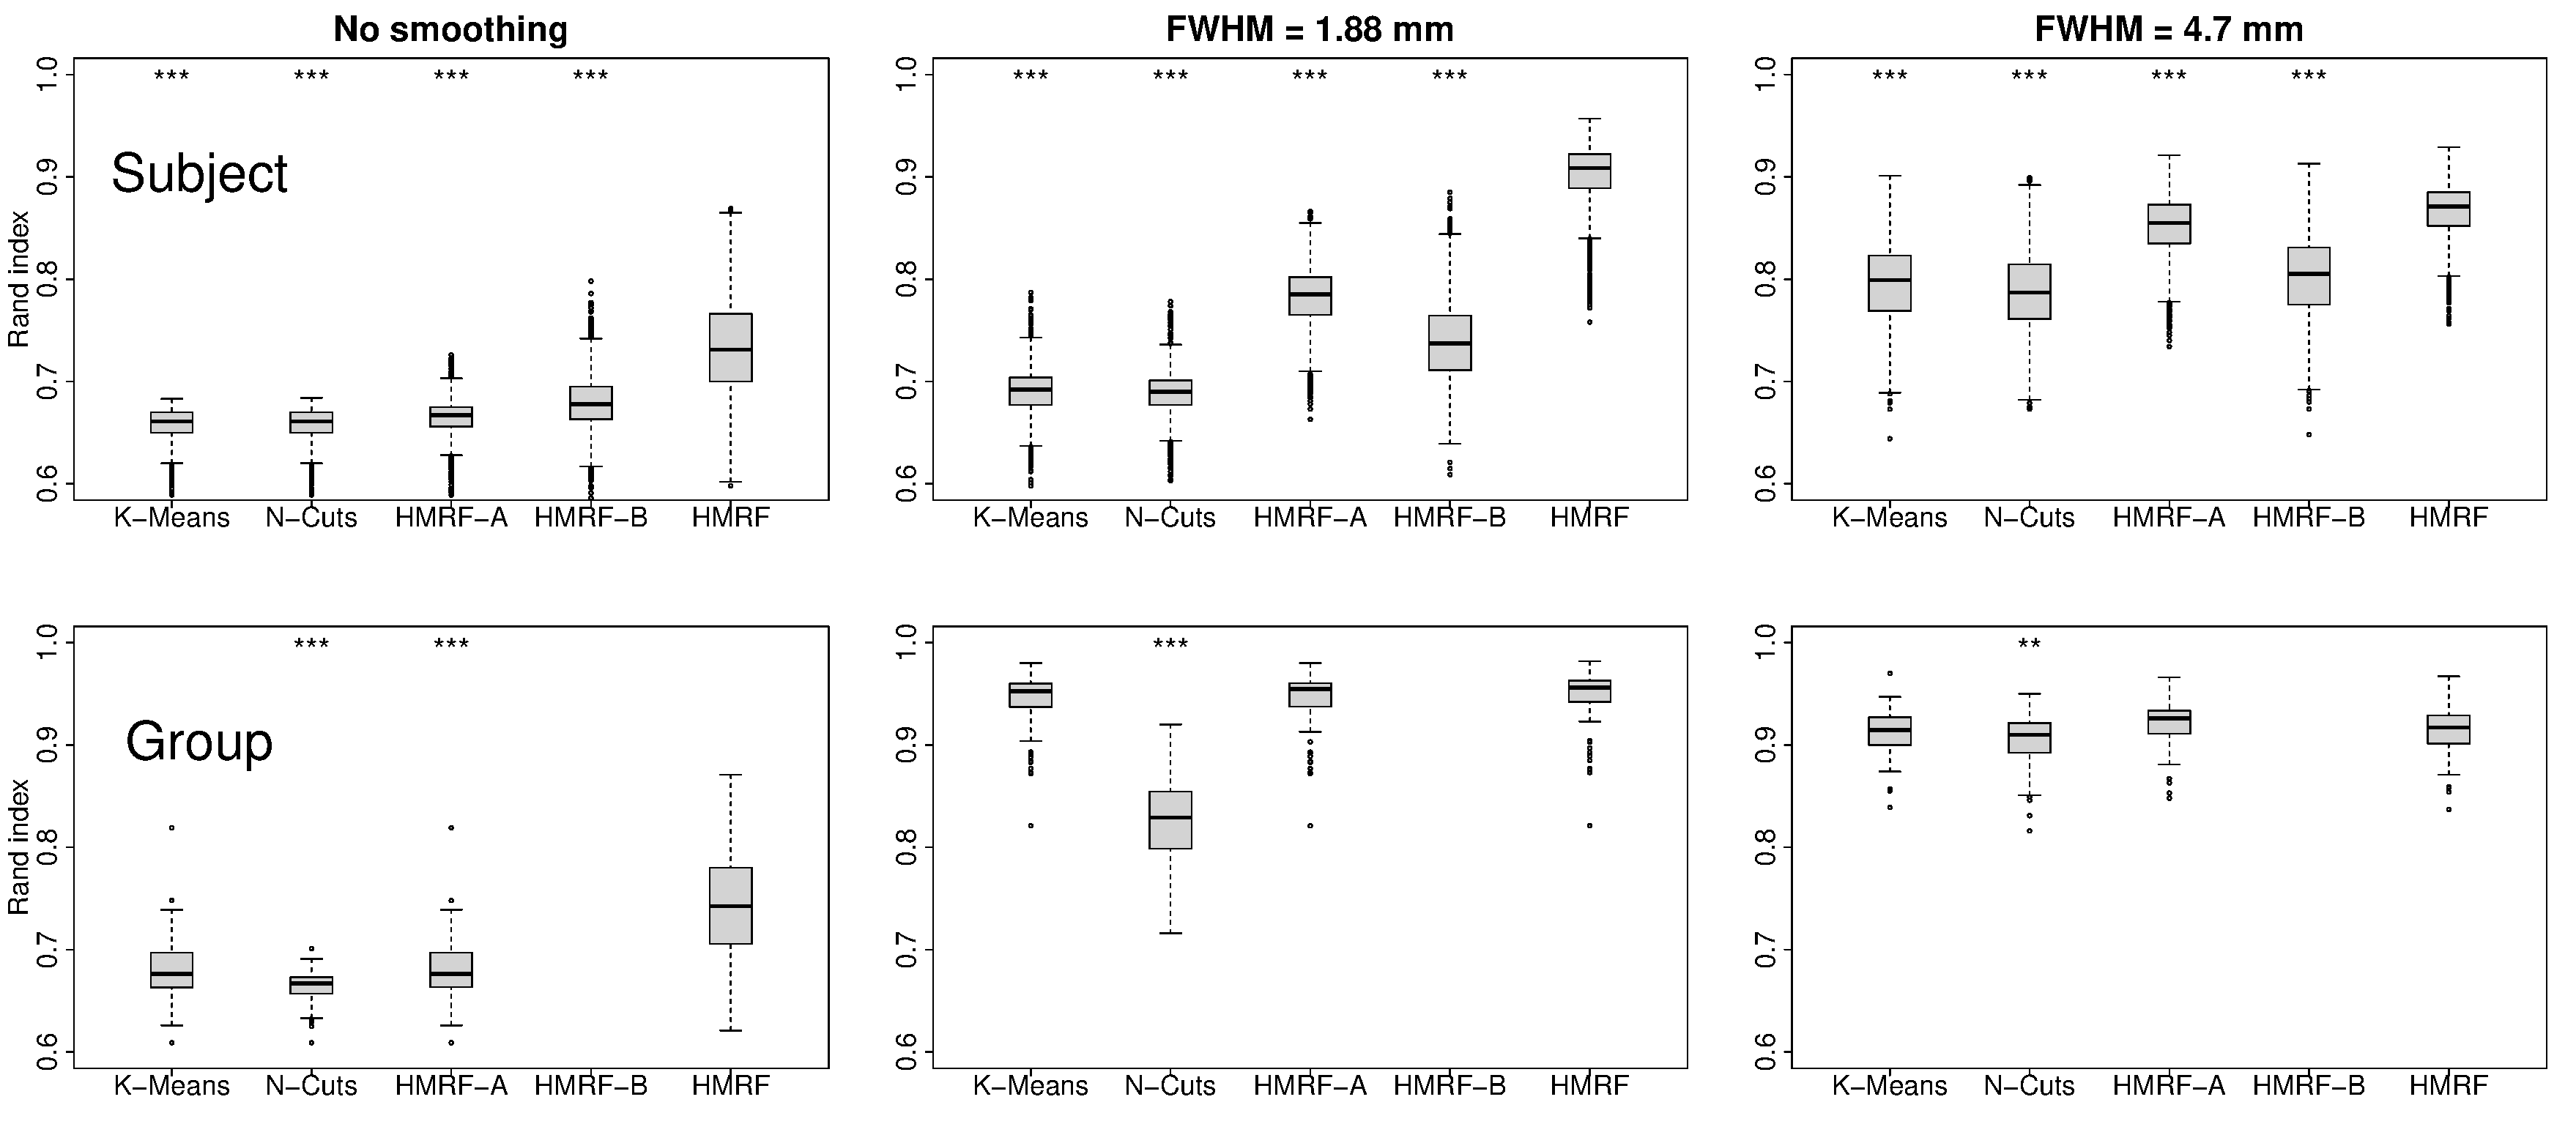
\includegraphics[width=1.0\textwidth]{figures/syn/2level_3smoothing}
  \caption{Box-and-whiskers plots of the estimation accuracies of all methods
    for three levels of spatial smoothing. The top row is the accuracies of
    subject labels across all subjects and MC samples, and the bottom is group
    map accuracies across all MC samples. The upper and lower 'hinges'
    correspond to the $25$th and $75$th percentiles. The asterisk on top of each
    box indicates the p-value of the standard two-tailed T test between HMRF and
    the corresponding method. No asterisk: significant $p > 0.05$; $*$:
    significant at $p < 0.05$; $**$: significant at $p < 0.01$; ${***}$:
    significant at $p < 0.001$. The group map is not applicable to \emph{HMRF-B}
    due to its lack of between-level links.}
  \label{fig:synboxplot}
\end{figure*}

% Interpreting the results. This part need very careful working. (unfinished)
To quantitatively evaluate the accuracy of the segmentation map from various
methods, we calculate the RI values between the true map and the estimated
map. The boxplot in Figure \ref{fig:synboxplot} shows the RI across all Monte
Carlo runs and subjects. In all three settings of smoothing kernel size, HMRF
achieves higher accuracies compared to other methods. In addition, for
individual subjects' estimation, our model performs best at a moderate smoothing
size of FWHM = 1.88 mm, which is smaller than the typical 5-8 mm smoothing
size. This is because the HMRF model benefits from the reduced noise variance
resulting from the moderate smoothing, but avoids losing finer details due to
excessive smoothing. In practice, this means when applying HMRF, the BOLD signal
should be smoothed by a small-kernel Gaussian filter, and we choose FWHM = 1.5
mm in the following real data experiments. We also note that the K-Means optimal
smoothing kernel size is larger than that of HMRF, because it lacks the spatial
coherence regularization and hence needs more smoothing in preprocessing
stage. Last, we found that the two reduced models HMRF-A and HMRF-B do not
perform as well as the full model, indicating that the hierarchy in the full
model is indeed necessary. For all possible smoothing sizes, HMRF's estimation
accuracy is comparable or moderately better than the other four methods on the
group label map, and significantly higher on subject maps.

\section{Real Data Experiments}
\label{sec:realexperiments}
% why use this data.
In this work we test our methods on the publicly available NYU test-retest (TRT)
dataset that has been used previously by \citet{shehzad2009resting} and
\citet{zuo2010reliable}. While the original goal of the above works was to
verify the voxel-wise intra- and intersession TRT reliability, our goal is to
verify whether the methods under consideration are able to estimate consistent
functional network maps across sessions, given the fair amount of intersession
consistency in the data
set~\citep{damoiseaux2006consistent,chen2008group,meindl2010test,franco2009interrater}. We
present two experiments with the NYU-TRT datasets. The first experiment aims at
demonstrating the intersession consistency of the estimated subject network
maps, and the second one evaluates how the algorithms behave under the
perturbation of the data by using bootstrap sampling. We compare three methods,
HMRF, K-Means, and N-Cuts, in both experiments. The other two methods, HMRF-A
and HMRF-B, are not taken into account in this section since they are a
simplified version of HMRF and have been shown to be suboptimal compared to the
full model.

\subsection{Preprocessing}
% How the data is generated.
Twenty-six healthy control participants (11 males, mean age 20.5 $\pm 4.8$
years) were scanned three times. The participants had no history
of psychiatric or neurological illness. BOLD EPI images (TR = 2 s, TE = 25 ms,
flip angle = 90, 39 slices at 3 mm slice thickness, 64$\times$64 matrix, field
of view = 192 mm, 197 volumes) were acquired on a Siemens Allegra 3.0 Tesla
scanner. Scans 2 and 3 were conducted in a single session, 45
minutes apart, and were 5-16 months after the first scan. The subjects were
asked to relax and remain still with their eyes open during the scan. A high
resolution T1-weighted image was also obtained (MPRAGE with TR = 2.5 s, TE =
4.35 ms, TI = 900 ms, flip angle = $8^\circ$, 176 slices, FOV = 256 mm).

The fMRI data was preprocessed using the scripts of the 1000 functional
connectomes
projects \footnote{\url{www.nitrc.org/plugins/mwiki/index.php/fcon_1000:ScriptUse}},
as well as FMRIB's FSL toolset and the Medical College of Wisconsin's AFNI
tool \footnote{\url{http://afni.nimh.nih.gov}}. The volumes are motion corrected
by aligning to the mean volume with a six-parameter rigid body
transformation. The BOLD signals were bandpass filtered to 0.01 to 0.1 Hz, and
were regressed out nuisance variables including white matter, CSF mean time
courses and six motion parameters. The signal is then filtered by a FWHM = 1.5
mm Gaussian filter for spatial smoothness. The small kernel size of spatial
smoothing helps increasing the SNR without introducing
blurring artifact on the functional network patterns (see the simulated test and
Figure \ref{fig:synboxplot} for the rationale of choosing small FWHM). The
functional images are first registered to the corresponding T1 images, and both
functional and T1 images are registered to MNI152 (Montreal Neurological
Institute) space with a 12-parameter affine transformation. Finally, after
masking out white matter and CSF voxels, we have 39080 gray matter voxels
remained in each subject. We construct a joint graph with over one million nodes
including all subjects and the group map.

\subsection{Choosing Parameters}
In this work we do not address the problem of how many functional networks exist
in the human brain. Instead, we use existing reports \citep{yeo2011organization}
and choose seven functional networks for segmentation throughout the real data
experiments. With this setting, we expect to identify the following typical
functional networks: visual and primary motor~\citep{damoiseaux2006consistent},
attention~\citep{fox2006spontaneous}, default mode network
(DMN)~\citep{greicius2004default}, saliency, and executive control
system~\citep{seeley2007dissociable}, regardless of the segmentation methods
used.  The K-Means is repeated 20 times with random initialization
\citep{arthur2007k} for segmentation of both the subject and group maps. For
N-Cuts, we threshold each subject's correlation matrix at 0.4 before applying
N-Cuts on single subject. After the individual segmentation, we average all
subjects' binary segmentation matrices, and threshold the averaged matrix at
0.3. The result represents the group correlation matrix. Both cut-off thresholds
are suggested by \citet{van2008normalized}. Our implementation is different with
from \citeauthor{van2008normalized} only in that we partition the subject map
into seven clusters instead of 20. This is because we need to compare the
subject maps estimated by N-Cuts with those estimated by the HMRF method at the
same number of networks. We also run N-Cuts with 20 clusters on subject maps to
compare with our seven-cluster configuration (results now shown), and find the
group level segmentation has not been impacted by our lack of over-segmentation
at the subject level. For HMRF, we initialize both the group and subject label
maps with the group label map estimated from K-Means. The sampling routine
(E-step of MCEM algorithm) skips 500 burn-in samples before saving 100 MC
samples. The parameters $\{\beta$, $\mu, \kappa\}$ are estimated from the
data. With $\alpha$ estimated from the posterior predictive distribution (see
section \ref{sec:alpha}), we found the similarity between estimated group and
subject maps measured is around 0.85 measured by RI value.

\subsection{Intersession Consistency}
% Discuss the inter-session experiment results.
Since the TRT dataset and the general rs-fMRI data have been shown to share
consistent functional networks across all
sessions~\citep{damoiseaux2006consistent, chen2008group, meindl2010test,
  franco2009interrater}, we verify the consistency of the HMRF algorithm by
applying it to each of the three sessions of data separately.  A method is said
to be consistent if it is able to derive similar network estimates across
sessions.  We compare three pairs of sessions' consistency: S1 vs S2, S1 vs S3
and S2 vs S3. For each subject in each pair of sessions, we compute the
consistency score between this subject's network map estimates in two
sessions. The similarity is again represented by the RI values. We expect the
proposed HMRF algorithm has higher average similarity compared with other
methods. The consistency scores of all subjects are summarized in a boxplot as
in Figure \ref{fig:sessionbox}. For comparison, the same boxplots are also drawn
for group ICA, K-Means and N-Cuts. For ICA, We use GIFT ICA
toolbox\footnote{http://mialab.mrn.org/software/}, with number of component set
to 7 and 25 respectively, and convert the overlapped spatial maps to discrete
labels by selecting the component with the strongest signal at each voxel. The
discretization of ICA map may lose information compared to Zuo et al.'s
intra-class correlation metric~\citep{zuo2010reliable}, but makes it possible
that all four methods are compared by same RI metric.

From Figure \ref{fig:sessionbox}, the subject network label maps estimated from
HMRF have significant higher intersession consistency scores compared to the
other three methods. This indicates that our algorithm is able to capture the
common functional patterns across sessions. In addition, K-Means, ICA and HMRF
have higher intersession consistency scores between session two and session
three, compared to the other two intersession comparisons. This is consistent
with the fact that sessions two and three have a smaller interval (45 minutes
apart), compared to session one and two (5-16 months). K-Means has slightly
better between-session consistency than N-Cuts, probably because we have run
K-Means multiple times and have chosen the best solutions. On the group level,
the HMRF label maps have intersession RI value of 0.917, 0.908 and 0.893 between
each pair of sessions, comparable to other methods.

% Here also need to give the p value asterisk information.
\begin{figure*}[htb]
  \centering
  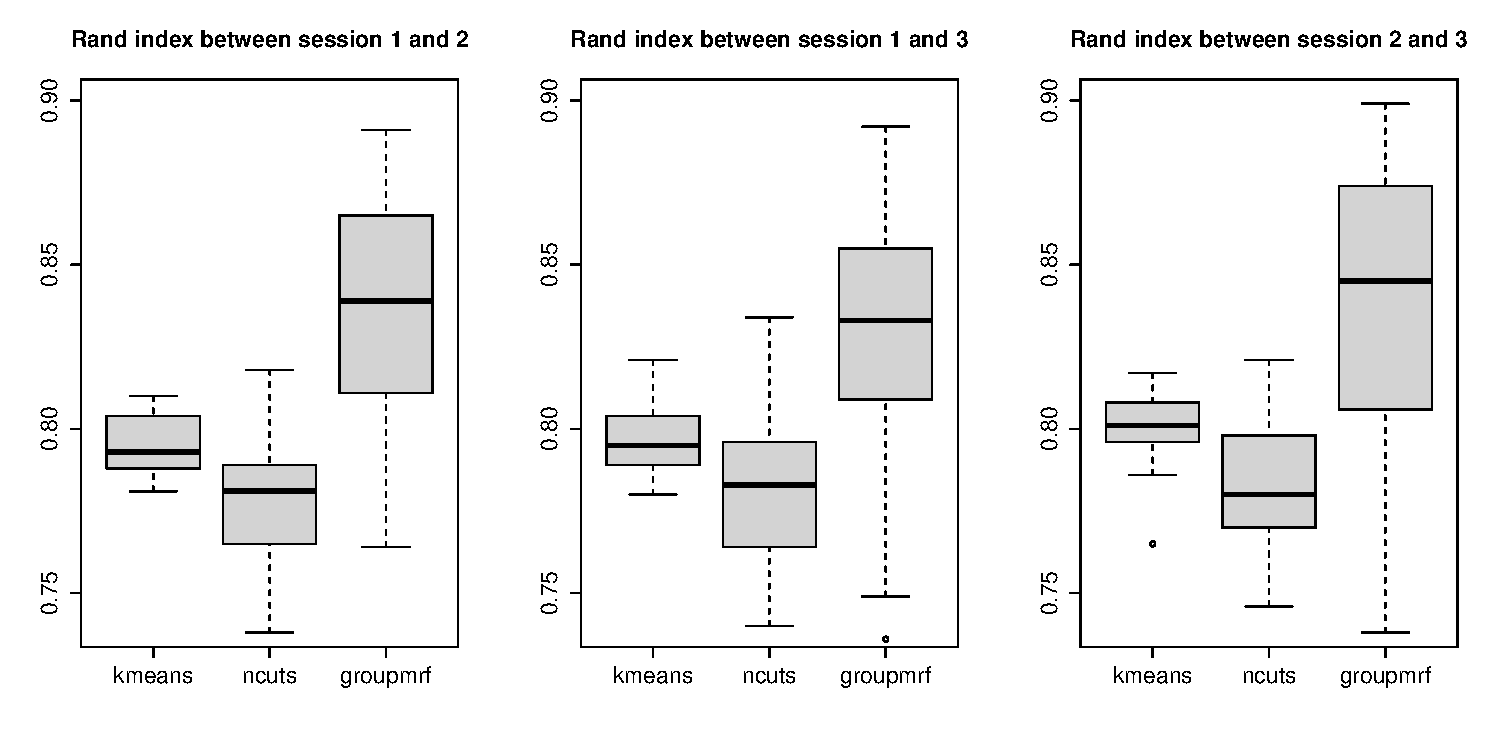
\includegraphics[width=0.9\textwidth]{figures/rainlog/boxplot}
  \caption{Box-and-whiskers plots of the RI value between each pair of
    sessions over the all subjects' label map. The bottom and top of the boxes are
    the $25$th and $75$th percentile, and the whiskers extend to the whole
    range of the data except the outliers.}
  \label{fig:sessionbox}
\end{figure*}

The RI values in Figure \ref{fig:sessionbox} only gives a single number of
similarity between two network label maps, rather than a voxel-wise consistency
map. To visualize the consistency at the voxel level, we first match session two
and session three's segmentation maps to session one's by permuting the cluster
labels (this is not needed for the between-session RI, which is invariant to
label permutation).  Then we define a variance map as follows: the variance at
certain voxels takes the value 0 if the estimates of all three sessions have the
same labels. The variance takes 1 if two of the three sessions have the same
labels, and takes 2 if none of the estimates are the same. We then average the
variance map across all subjects and obtain a mean variance map. This map shows
how the algorithm performs in term of consistency at the voxel level across all
subjects. The results are shown in Figure \ref{fig:intersessionvar}.  Image
visualization is done by using nipy, a python package for neuroimaging
data~\footnote{http://nipy.org/nipy/stable/index.html}. We note that
although K-Means and N-Cuts have low variance at the visual cortex, they have
larger variance in most voxels of dorsal attention and the DMN. These findings
confirm the different level of consistency between the functional networks, as
has been shown in the original work of~\citet{zuo2010reliable}. Overall, the
HMRF method's estimates have the lowest level of variance and hence the highest
level of consistency.

\begin{figure*}[htb]
  \centering
  \includegraphics[width=1.0\textwidth]{figures/012map/012variance}
  \caption{The intersession variance maps estimated by four methods. ICA-7 and
    ICA-25 denote ICA with 7 and 25 components, respectively. The variance maps
    are obtained for each subject, averaged across subjects, and finally
    normalized to [0, 1]. A few voxels with intensity above 0.8 are rendered the
    same as those with intensity 0.8. This single map covers all seven
    functional networks, and we selectively show the slices corresponding to the
    three major networks. The images left are the subjects' left, and we use the
    same convention in the following figures. }
  \label{fig:intersessionvar}
\end{figure*}

\subsection{Bootstrapping}
%% Add bootstrap experiment setup here. First we need a short intro of
%% bootstrap.
In these experiments we aim to evaluate the performance of the three algorithms
with bootstrapping. In the bootstrapping method, one covers the whole
distribution of the estimator with the independent samples drawn from the
original dataset with replacements, and estimates the stability of an
algorithm~\citep{efron1993introduction}. An approximate solution of an algorithm
is stable if the solution is not highly sensitive to the input data. It is
unstable if a slight change in the data can cause the predicted values to change
significantly. In this experiment, the bootstrapped samples can be seen as a
small perturbation of the input data and will be used to test the algorithm
stability.

There are various approaches for resampling the available data. One may resample
the subjects from the original dataset~\citep{damoiseaux2006consistent}. Here
for each voxel of each subject in session 1, we sample with replacement from the
197 time points of preprocessed data, and obtain a bootstrap sample volume with
the same BOLD signal length and number of subjects with the original
dataset. The sampling is similar to the circular block bootstrap  in
\cite{bellec2010multi}, except that we do not model the temporal correlation
between time points. Since all methods under comparison here do not model
temporal correlation, the shuffling of the time points has no effect on the
segmentation results.  After repeating the sampling 100 times, we obtain a set
of 100 bootstrap samples, each of which includes all subjects' time series
data. Then, all three segmentation methods are applied on each of the bootstrap
datasets. We estimate group and subject level maps from each bootstrap dataset
by using the three methods. All the estimated label maps are postprocessed by a
label permutation routine to guarantee that the same networks have the same
labels.

\begin{figure*}[htb]
  \centering
  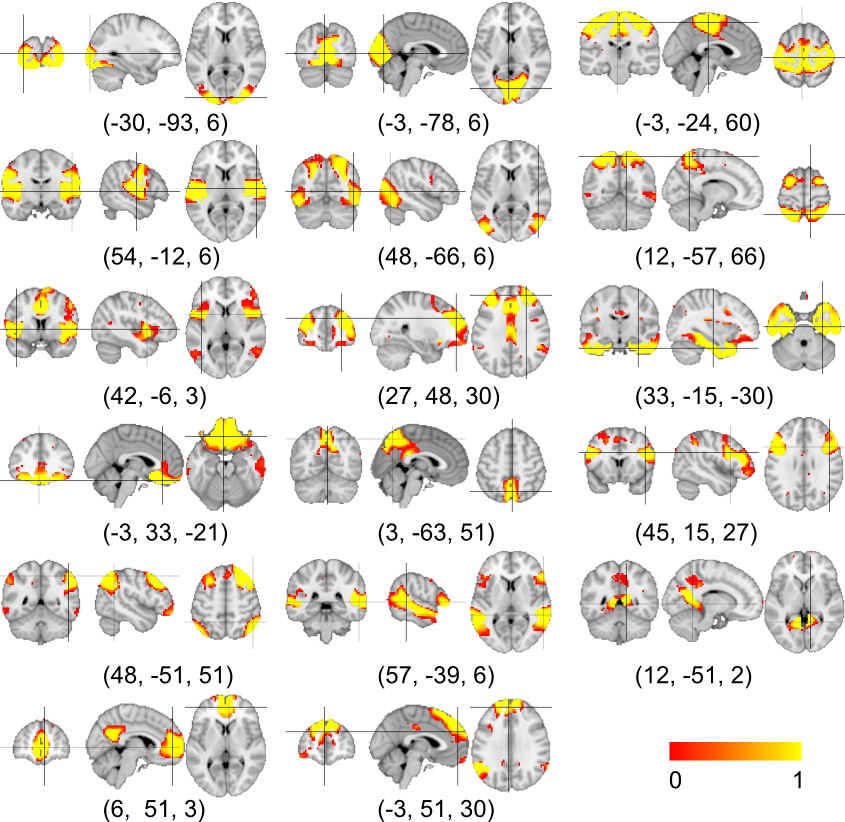
\includegraphics[width=0.9\textwidth]{figures/groupmean/grp_mean}
  \caption{The group level's mean functional networks estimated from all
    bootstrapped data by three segmentation methods. The binary maps of each
    network are averaged over all bootstrap samples. The average intensity ranges
    from 0 to 1.}
  \label{fig:grpmean}
\end{figure*}

\begin{figure*}[htb]
  \centering
  \includegraphics[width=0.9\textwidth]{figures/varmap/grp_var}
  \caption{The group variance map estimated from all bootstrap samples by the
    three segmentation methods. The variance values range from 0.05 to 0.25, but
    only those voxels in [0.05, 0.15] are shown for visualizing the difference
    of the methods under comparison.  }
  \label{fig:grpvar}
\end{figure*}

\begin{figure*}[htb]
  \centering
  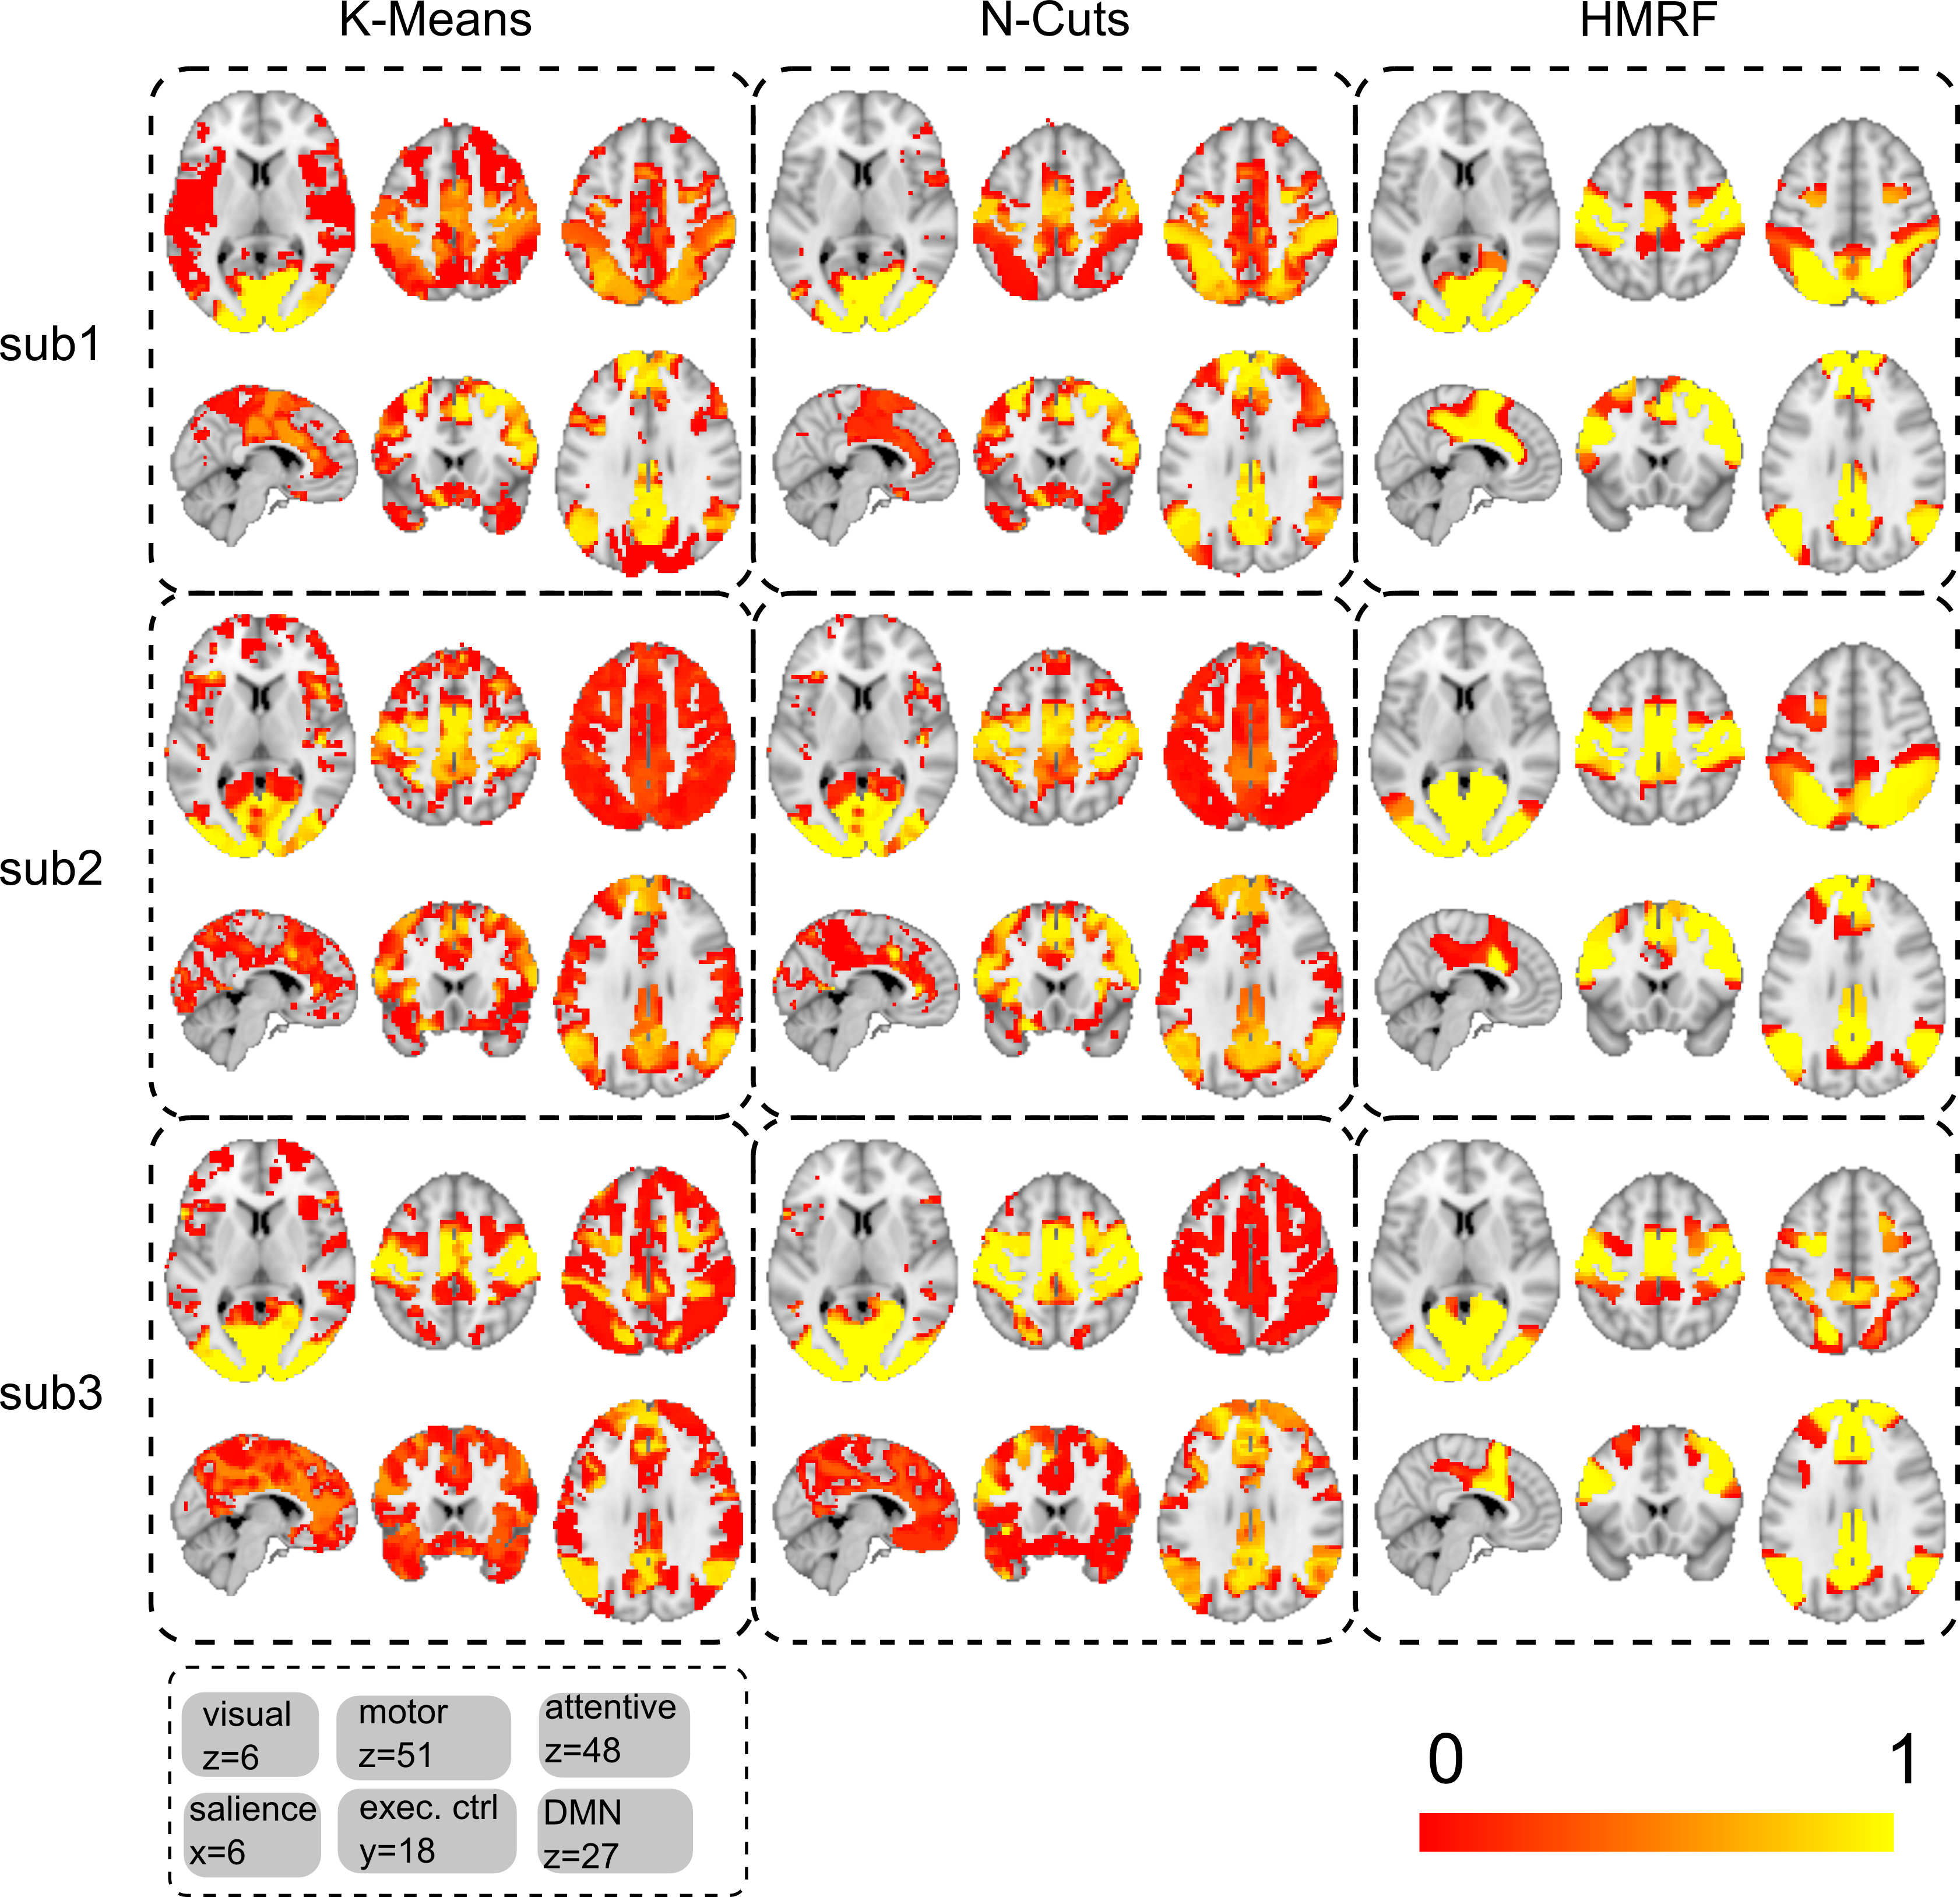
\includegraphics[width=0.9\textwidth]{figures/submean/submean}
  \caption{The three subjects' average network label maps estimated from all
    bootstrap samples. One representative slice is shown for each of the seven
    networks for each subject(row) and each method (column), excluding brain
    stem component. The average values range from 0 to 1. }
  \label{fig:submean}
\end{figure*}

\begin{figure*}[htb]
  \centering
  \includegraphics[width=1.0\textwidth]{figures/varmap/sub_var}
  \caption{The variance of the functional network maps of all subjects. The maps
    are averaged across all subjects and bootstrap samples. The variance values
    range from 0 to 0.25, but only those voxels in [0.05, 0.15] are colored to
    display the difference of the methods. }
  \label{fig:subvar}
\end{figure*}

% Analyze the results of bootstrapping.
Figure \ref{fig:grpmean} shows seven average group-level functional network maps
across all bootstrap sampled data. For each network, we extract a binary map
with voxel intensity taking 1 in that network and 0 outside. This binary map is
then averaged over all bootstrap samples. We also show the variance of this
binary label map over all samples in Figure \ref{fig:grpvar}. Small variance
indicates more stability under bootstrap sampling.  All three methods have
moderate to high stability across bootstrap samples. For visual, motor, and DMN
networks, K-Means and N-Cuts have reasonably high stability, although some
voxels at the boundary of the network regions are labeled differently across
bootstrap samples. For the attention, salience and executive control networks
estimated by K-Means and N-Cuts, the ambiguity not only happens on the boundary
of the network regions, but also on some bigger regions inside the networks. For
example, in some bootstrap runs, K-Means incorrectly assigns the posterior
cingulate cortex (PCC) to the attentive network (see the red regions in dorsal
attentive in Figure \ref{fig:grpmean}), whereas PCC has been shown to be part of
the DMN~\citep{greicius2003functional}. K-Means also miss part of the primary
motor network, and merges the voxels in limbic system into the DMN in a few
bootstrap runs. For N-Cuts, the dorsal attentive, salience, and executive
control networks have larger variance under this data perturbation. Compared to
the other two methods, HMRF has significantly smaller variance as indicated by a
two-tail t test with significance level 0.01, and hence the highest stability
in all seven networks. A small number of voxels in motor and DMN still shows
unstable assignments.

% discuss mean and variance map on subject level, which is more interesting than
% the group.
To demonstrate the stability of the estimates on each of the subject functional
networks, we first pick 3 subjects from the 25 subjects in the dataset. For each
subject, we show the average network patterns over all bootstrap samples. See
Figure \ref{fig:submean}. We show only six major functional networks, excluding
the one corresponding to the limbic system. For each network, one representative
slice is shown. From the figure, all three subjects' mean network maps have
lower stability compared to their corresponding group networks. Certain
subjects' networks are significantly less stable than other subjects, due to the
various degree of perturbation by the random sampling even using the same
bootstrapping procedure. Among the six networks, attentive networks exhibit the
most dramatic change under bootstrap sampling. Some voxels of salience and
executive control networks are absorbed into attentive networks. This
mis-classification happens most on subject 2, and also happens a moderate amount
on subjects 1 and 3. Compared to the other two methods, HMRF is able to estimate
reasonably stable functional networks even with data resampling. Attentive
networks and executive control networks tend to change more than other networks,
but still less than K-Means and N-Cuts.

% Subject variance map.
Another way to show the stability of the subject label maps is the variance
map. Since we are interested in comparing among three methods the variance of
the networks across all subjects, we show the variance not for each single
subject, but an average variance over all subjects. See Figure
\ref{fig:subvar}. Because of the averaging over all subjects, the variance is
more spread over the voxels. Again, HMRF shows significantly smaller variance
than the other two methods in a t test at a significance level 0.01, indicating
its subject map estimates are more stable under bootstrap sampling.

% alpha estimation starts here.
\subsection{Between-Level Links estimation}
\begin{figure}[htb]
  \centering
  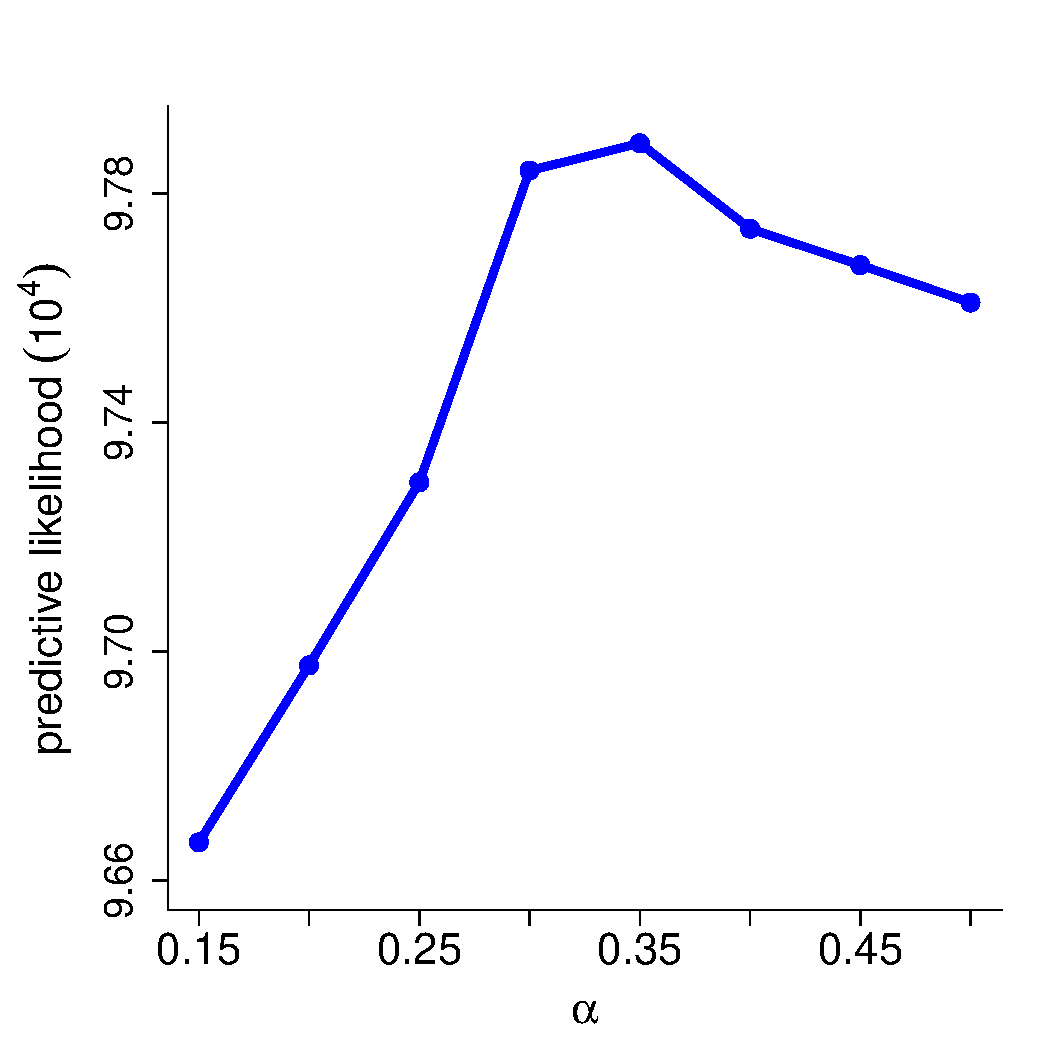
\includegraphics[width=0.5\textwidth]{figures/alpha/predictLLvsAlpha}
  \caption{Estimation of parameter $\alpha$ with the average predictive
    distributions using the leave-one-out cross-validation. We use the data from
    only the first session of the NYU-TRT dataset but find similar patterns in
    the other two sessions. $\alpha$ are sampled between 0.15 and 0.5, with
    interval 0.05.}
  \label{fig:alphaest}
\end{figure}

We also run the cross-validation and use the posterior predictive distribution
in equation \eqref{eq:valalpha} for estimating the optimal $\alpha$
parameter. Figure \ref{fig:alphaest} gives a plot of the average predictive
density with alpha ranging in [0.15, 0.5], with interval 0.05. We found that with
too small $\alpha$, the model has low prediction values on the test data, and
too large $\alpha$ values improve the prediction but still not the optimal. The
best $\alpha$ value is around 0.3 to 0.35.

\section{Discussion}
\label{sec:discussion}
We proposed a new hierarchical model for identifying functional networks of the
human brain from a group of rs-fMRI dataset. The model assumes a group
functional network map is shared among all subjects in the population, and
individual subjects' functional patterns are generated as variations from this
group level network. If we see the functional network pattern as a clustering of
the fMRI data, we actually assume the subject maps are samples from an unknown
distribution of the clusterings, with its mean given by the group map. We
reformulate the distribution of clusterings as a distribution of network labels,
where a subject's labels at each voxel are seen as generated from the group's
network labels. While the intersubject statistical dependency is defined by the
links between group and subject labels, the spatial coherence of the functional
networks is guaranteed by the within-subject MRF. All the network label
variables at both levels with their links, along with the parameters are defined
in an integrated graph, and the general techniques of graphical models can be
used for (approximate) inference. This multilevel view is typically used in
general statistical analysis when the individuals are grouped into units, and
the variance of the variables is decomposed into the group-specific and
subject-specific terms. We borrow the multilevel view and apply it to the
clustering problem where the intensities of voxels at each time point are
grouped into units (subjects), and the vMF's $\kappa$ parameter represents the
individual subject's variance. The $\alpha$ parameter is equivalent to the
\emph{pooling factor} in the standard hierarchical linear
model~\citep{gelman2006bayesian}, and controls the degree to which the estimates
of subject label maps are pooled together.

We use the MCMC sampling for the inference because of its good approximation of
the posterior density. An alternative class of methods is variational inference,
including mean field approximation and expectation propagation. Both variational
methods and MCMC are the approximation of the true posterior
distribution. Variational inference approximates the target distribution by the
product of factorized distributions, while the sampling approximates the
posterior distribution by Monte Carlo averaging. Both classes of methods depend
on initial conditions. The derivation of the conditional expectation
used for the update of variational methods would be cumbersome in our multilevel
model. On the other hand, the Gibbs sampling is straightforward as the
conditional probability is easy to compute in our Bayesian setting. Therefore,
we choose Gibbs sampling due to its simplicity, as well as the fact that the
application does not require real time computation. An additional critical
property of the MCMC sampling is that its convergence does not depend on the
dimension of the variables~\citep{robert2005monte}; thus we can achieve
reasonable compute time even in this million-dimensional problem. The whole
Monte Carlo expectation maximization procedure uses 45-50 cores on a
multiprocessor machine, and takes about 2 hours for a group of 25 subjects.

% Spatial smoothing necessary
As a practical guide for applying HMRF, the introduction of within-subject MRF
is not meant to replace the spatial smoothing in the preprocessing steps. This
is one step further from what we found in our previous
work~\citep{liu2012group}, where no spatial smoothing is conducted when the HMRF
model is used. We found a moderate spatial smoothing, plus our HMRF model can
achieve the best estimation accuracy in the simulated experiments, and the best
consistency in the real data experiments. The good performance of the combined
moderate smoothing + HMRF model is because that moderate smoothing increases SNR
without overly modifying the signal and risking losing patterns at finer
scales. The MRF regularization further favors spatial coherence and intersubject
coherence.

The HMRF model defines a mixture of vMF distribution on the observed BOLD data,
and is inherently an image segmentation method. Therefore, the model inherits
the limitations of the mixture model. For example, the number of clusters are
given \emph{a priori}, as the widely-accepted method of estimating this number
is not available. For 7, or even 17 functional networks suggested by
\citet{yeo2011organization}, different networks may have been merged into a
single cluster (see Figure 1-4 in the supplementary material for the
results of 17 networks). Another limitation is the assumption that all gray matter voxels
are part of certain networks, which may not reflect the true functional
organization. Some voxels may not participate any spontaneous activity, hence
residing outside of any functional network. Additional modeling techniques are
needed to identify those \emph{background} voxels. Similar to ICA-based
methods, each voxel is assumed to belong to a single functional network. While a
large number of brain regions appear to have single functional pattern, studies
show that some regions, such as the precuneus, have a wide spectrum of highly
integrated networks, including visuo-spatial imagery, episodic memory and
self-processing operation~\citep{cavanna2006precuneus}. These voxels with
overlapping functional patterns remain a challenge to segmentation-based methods
including HMRF, despite that the posterior distribution helps the estimation to
some extent. Last, our model moderately accounts for intersubject variation. So,
it may have difficulty dealing with subjects whose functional network topology
is fundamentally different from the group average, for example, a subject who
has had neurosurgery. 

On the experimental side, we showed the increased consistency of the HMRF model in
intersession and bootstrap tests, but note that consistency is not the only
metric of evaluating the models. By regularization on the subject networks, we
risk of losing variability on the subject map, such that the subject maps
estimated by HMRF may not represent the true underling functional patterns of
each subject. The estimation of the between-level link parameter $\alpha$ by
Bayesian cross validation is one attempt to mitigate the possible
over-regularization (see Figure 5 in supplementary material for a comparison
with seed-based correlation analysis).

% revision: phenotype relationship. 
One interesting question is what impact that our HMRF model has on the possible
correlation of the functional connectivity as a phenotype and other variables of
interest. To test this hypothesis, we use both age and sex as independent
variables, and use them to predict the functional network labels estimated by
the non-hierarchical model (such as K-Means) and HMRF respectively. As each
voxel is tested for possible correlation independent of other voxels, we count
the number of voxels significantly correlated with age or sex for network maps
of both K-Means and HMRF. The results in Table 1 and Table 2 of the
supplementary material show that the percentage change in number of voxels
range from -2.68\% to 2.75\% over all six functional networks and two
independent variables, and mostly are within $\pm 1\%$. The decreased number of
significant voxels using HMRF is because the subject network maps shift towards
the population network map. The increased number of voxels for certain networks,
is because new correlations emerge after the HMRF model recovers more
accurate network maps. The small percentage of changed voxels indicates
the limited impact of HMRF on the possible phenotype correlation, though more
sophisticated approaches, such as \citet{alexander2012discovery}
 and \citet{reiss2012paradoxical}, will be needed to elucidate whether HMRF model
illuminate or diminish the network-phenotype relations. 

Overall, our model is an attempt to extract more reliable functional network
patterns from multi-subject datasets. The hierarchical concept in our
methodology makes sense on today's large imaging repositories such as the human
connectome project, the 1000 functional connectome project, and the Autism brain
imaging data exchange project. Because of a wider range of subject groups with
different pathologies~\citep{smith2012future}, the data in these projects has
even greater heterogeneity of scanning parameters than single-site data, despite
efforts toward strict quality control process~\citep{marcus2013human}. Our model
fits the hierarchical site-subject nature of the data acquisition process and is
able to account for the heterogeneity in the data. With more reliable estimation
of the functional network patterns as imaging phenotype, our model may also
reveal more genotype-phenotype interaction at the subject level by using large,
lower-quality datasets. Equally encouraging is the application of our model
towards a more robust characterization of single subject results, a critical
step needed for clinical applicability of resting state functional
connectivity. With improved single subject functional network parcellations, it
may be possible to achieve diagnostic and prognostic classifications that can
inform clinical management in dozens of neurological, neuropsychiatric, and
neurodevelopmental disorders to which fcMRI has been applied, and further work
could establish whether HMRF processed data may enhance biomarker specificity
and sensitivity.

\section{Conclusion}
The main contribution of our work is a hierarchical model for estimating
population functional network maps as well as individual subjects' maps from
rs-fMRI data. The relationship of the network labels in both group and subjects
is represented probabilistically. We solve the multivariate inference problem by
MCEM sampling.  The results for a synthetic group of fMRI data show that our
method achieves higher accuracy on both group and subject network map estimation
than the regular \emph{one-way} approach, such as K-Means and normalized
cuts. The experiments on a multiple-session rs-fMRI dataset show that our HMRF
algorithm is able to estimate the network maps for each session with higher
between-session consistency. A further bootstrapping experiment also proves the
proposed algorithm has robust solutions under data perturbations.

\appendix
\section{Predictive Distribution}
\label{sec:appalpha}
The test subject's predictive distribution in \eqref{eq:valalpha} for a chosen
$\alpha$ can be evaluated through a Monte-Carlo approximation
\begin{align}
P(Y_t|X; \alpha; \theta_t) \approx \frac{1}{M}\sum_m P(X_t|Y_t^m; \alpha, \theta_t), \quad Y_t^m \sim P(Y_t|X; \alpha). \label{eq:alphaapp1}
\end{align}
One economical way of generating sample $\{Y_t^m, m = 1\dots, M\}$ can be done
within the MCEM loop of algorithm \ref{alg:alg1}. After the current group map is
generated in E step, one sample $Y_t^m$ can be generated from $P(Y_t|X; \alpha,
\theta)$. The corresponding posterior energy function at voxel $s$ is $U_p
(y_s|y_{ N(s)}) = \alpha \psi(y_s,y_{\tilde s}) + \beta\sum_{r\in N(s)} \psi
(y_s, y_r)$. This energy is same to equation \eqref{eq:engsub}, except that
there is no time series data term $\kappa_l \mu_l^{\intercal} x_s - \log C_p$
since the test subject data $X_t$ are not given in this distribution.  For one
sample map $Y_t^m$, the test subject parameter set $\theta_t$ is obtained by
optimizing $P(X_t | Y_t^m)$. As a simple reasoning of why we can use the equation
\eqref{eq:valalpha} for estimating $\alpha$, when $\alpha$ is too small, most of
the $Y_t^m$ will depend less on the group map $Y_G$ and tend to be random
clusterings, which will have low data likelihoods in \eqref{eq:alphaapp1}. When
$\alpha$ is too big, $Y_t^m$ will be almost the same as $Y_G$, again resulting
in a suboptimal value for \eqref{eq:alphaapp1}. Only with an appropriate
$\alpha$, could $Y_t^m$ sufficiently explores the sampling space including the
regions where the predictive distribution is maximized. In practice, we evaluate
eq. \eqref{eq:alphaapp1} for a fixed set of $\alpha$ values, and choose $\alpha$
with the largest predictive density value $P(Y_t|X; \alpha)$.

\bibliographystyle{model2-names}
\bibliography{myreference}
\end{document}

